\section{Color Balancing}
\subsection{Cumulative Histograms}
In this section I had to calculate and plot the cumulative histograms for the R, G and B components for kodim23a.png and kodim23b.png (Figure \ref{fig:KodimImages}). These histograms can be seen in Figure \ref{fig:KodimCumHistogram}

\begin{figure}[h]
    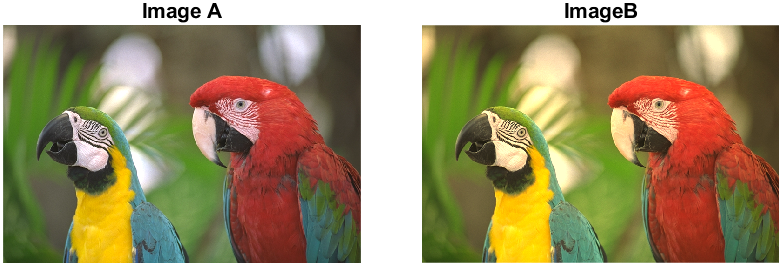
\includegraphics[width=1\textwidth]{KodimImages.png}
    \centering
    \caption{kodim23a.png and kodim23b.png}
    \label{fig:KodimImages}
\end{figure}

\begin{figure}[h]
    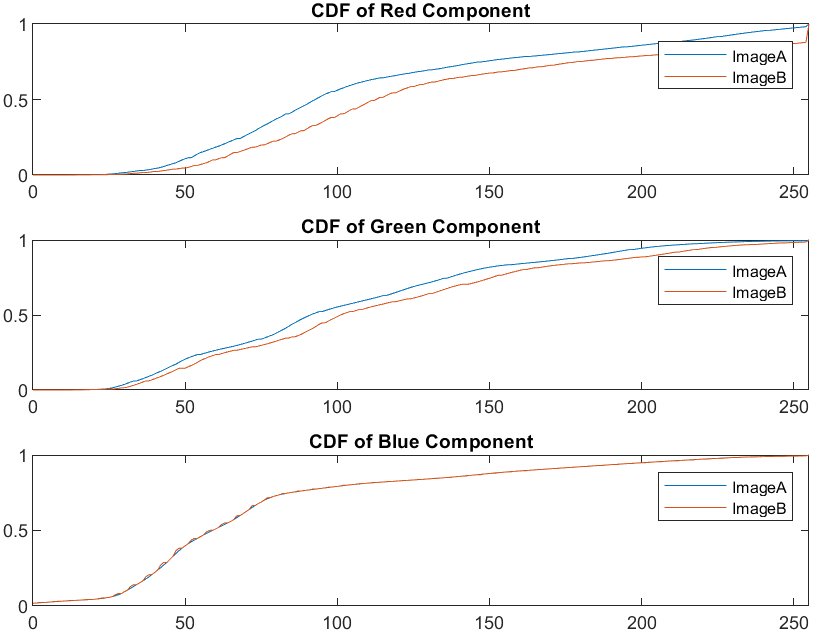
\includegraphics[width=1\textwidth]{KodimCumHistograms.png}
    \centering
    \caption{Cumulative Histograms for kodim23a and kodim23b}
    \label{fig:KodimCumHistogram}
\end{figure}

\subsection{Color Mapping Kodim23b to Kodim23a}
Using these histograms I calculated where the channel value of 150 in kodim23a got mapped to in kodim23b. These values were used to calculate the gray-point ($R_g, G_g, B_g$) of the image. From this the color mapping matrix can be calculated:
\begin{gather}
    \begin{bmatrix}
        R_a \\
        G_a \\
        B_a \\       
    \end{bmatrix}
    =
    \begin{bmatrix}
        \frac{150}{R_g} & 0 & 0 \\
        0 & \frac{150}{G_g} & 0 \\
        0 & 0 & \frac{150}{B_g}
    \end{bmatrix}
    \begin{bmatrix}
        R_b \\
        G_b \\
        B_b \\
    \end{bmatrix}
\end{gather}

\begin{gather}
    \begin{bmatrix}
        R_a \\
        G_a \\
        B_a \\       
    \end{bmatrix}
    =
    \begin{bmatrix}
        \frac{150}{182} & 0 & 0 \\
        0 & \frac{150}{167} & 0 \\
        0 & 0 & \frac{150}{150}
    \end{bmatrix}
    \begin{bmatrix}
        R_b \\
        G_b \\
        B_b \\
    \end{bmatrix}
\end{gather}

By performing this caluclation on all the pixels of the image, we can color match kodim23b to look more like Kodim23a. The result of performing this transformation can be seen in Figure \ref{fig:KodimTransform}, the average absolute error between Kodim23a and the transformed Kodim23b can be seen in Figure \ref{fig:KodimAAE}

\begin{figure}[!h]
    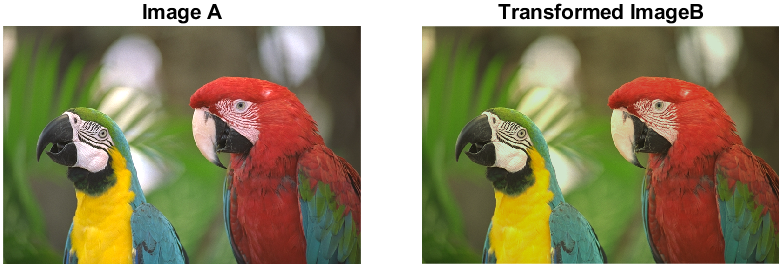
\includegraphics[width=1\textwidth]{KodimTransformed.png}
    \centering
    \caption{Tranformation of Kodim23b to color match Kodim23a}
    \label{fig:KodimTransform}
\end{figure}

\begin{figure}[!h]
    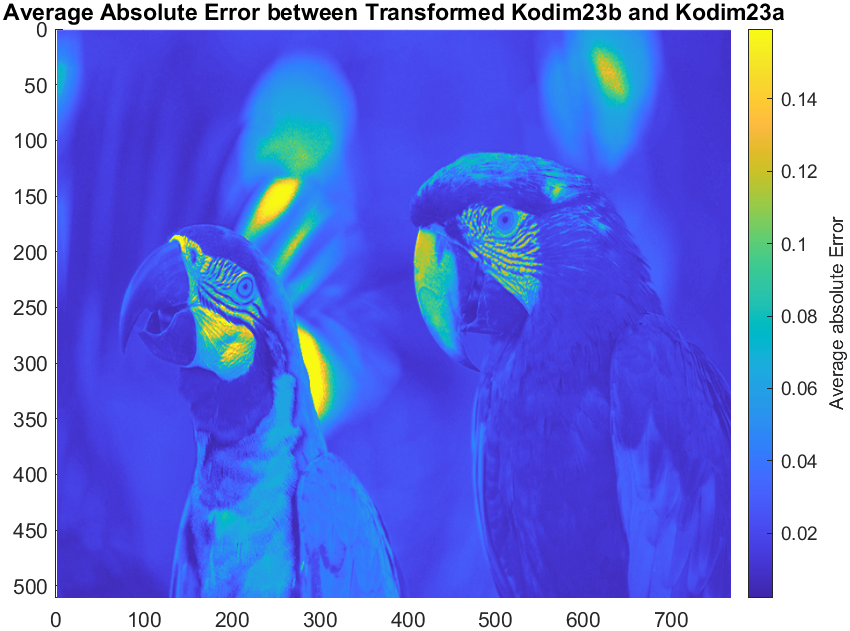
\includegraphics[width=1\textwidth]{KodimTransformedAAE.png}
    \centering
    \caption{Average Absolute error between Kodim23a and the transformed Kodim23b}
    \label{fig:KodimAAE}
\end{figure}
